\subsection{Using \textit{store} operations to observe presence/absence of victim traffic on PCIe}
\label{subsec:interconnect-sc-store-ops-measuring-time}
Now, we have a mechanism to issue multiple \textit{store} instructions in parallel while timing the completion of an individual (or a small group of) \textit{store} instructions.
We can use this mechanism and the threshold of $N = 81$ to observe the presence or absence of victim traffic in the PCIe controller.
To achieve this, we execute the pseudo-code outlined in \Cref{lst:timing-victim-with-stores} with the victim transferring a large amount of data to or from the GPU via DMA
\footnote{Since most GPU-based applications rely on the DMA controller for efficient transfers, we assume that the victim uses DMA.}.

To evaluate our ability to detect victim traffic, we run the adversary for $10^5$ iterations.
At the same time, we execute the victim, which repeatedly (for $10^4$ iterations) performs a DMA transfer of either 4KB or 4MB.
The 4KB transfer does not saturate the PCIe link, while the 4MB transfer saturates the PCIe link (see \Cref{fig:bw-util-and-time-per-size}).
Additionally, we synchronise the execution of the critical code sections responsible for data transfers between the victim and the adversary. 
This synchronisation allows us to measure whether we can detect the presence or absence of victim traffic, even though such perfect alignment is unrealistic for a side-channel attack.

As shown in \Cref{fig:cpu-store-victim-observation}, the execution time of the individual \textit{store} operations by the adversary increases in the presence of victim traffic, irrespective of whether the victim is saturating the PCIe link or not.
Without a victim, the \textit{store} instruction takes $<15~cycles$ to complete. However, in the presence of victim traffic, the execution time increases to $>15~cycles$ and drops again once the victim is done transmitting.
As such, an adversary can determine the presence/absence of victim traffic.
The adversary observes a fixed delay in the execution time of the \textit{store} instruction irrespective of the size of the data being transferred by the victim.
However, the duration for which the adversary observes the delay increases with the amount of data the victim transfers.
This is the case because the victim transfers the data using \textit{burst mode} of transfer, where the burst size is fixed.


% \begin{minipage}{\textwidth}
    \lstinputlisting[language=Python]{code/interconnect-sc/timing-victim-with-stores.py}
    \captionsetup{type=lstlisting}
    \caption{Pseudo-code to detect presence of victim traffic via \textit{store} instructions}
    \label{lst:timing-victim-with-stores}
% \end{minipage}

\begin{figure}[!htb]
    \centering
    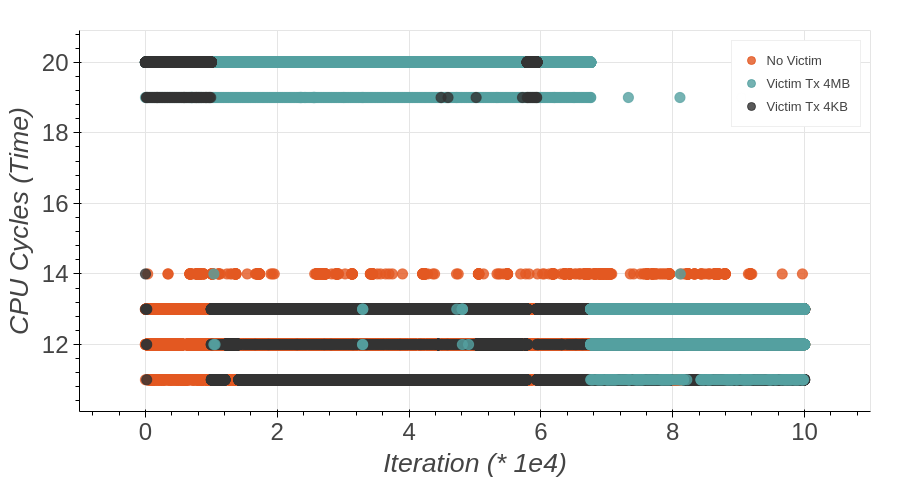
\includegraphics[width=\columnwidth]{figures/interconnect-sc/store-ops/cpu_store_victim_observation.png}
    \caption{The attacker can observe the presence of victim traffic using \textit{store} operations.
    The attacker observes the contention for more iterations or longer duration when the victim is transferring more data.}
    \label{fig:cpu-store-victim-observation}
    % 2025-03-06_14-20
\end{figure}
